\documentclass[11pt]{aghdpl}
% \documentclass[en,11pt]{aghdpl}  % praca w języku angielskim

% Lista wszystkich języków stanowiących języki pozycji bibliograficznych użytych w pracy.
% (Zgodnie z zasadami tworzenia bibliografii każda pozycja powinna zostać utworzona zgodnie z zasadami języka, w którym dana publikacja została napisana.)
\usepackage[english,polish]{babel}

% Użyj polskiego łamania wyrazów (zamiast domyślnego angielskiego).
\usepackage{polski}

\usepackage[utf8]{inputenc}

% dodatkowe pakiety

\usepackage{mathtools}
\usepackage{amsfonts}
\usepackage{amsmath}
\usepackage{amsthm}
\usepackage{xargs}                      % Use more than one optional parameter in a new commands
\usepackage[pdftex,dvipsnames]{xcolor}  % Coloured text etc.
\usepackage[colorinlistoftodos,prependcaption,textsize=tiny]{todonotes}
\usepackage[export]{adjustbox}
\usepackage{rotating}
\usepackage{float}
\usepackage{booktabs}
\usepackage{everypage}

\newcommandx{\unsure}[2][1=]{\todo[linecolor=red,backgroundcolor=red!25,bordercolor=red,#1]{#2}}
\newcommandx{\change}[2][1=]{\todo[linecolor=blue,backgroundcolor=blue!25,bordercolor=blue,#1]{#2}}
\newcommandx{\info}[2][1=]{\todo[linecolor=OliveGreen,backgroundcolor=OliveGreen!25,bordercolor=OliveGreen,#1]{#2}}
\newcommandx{\improvement}[2][1=]{\todo[linecolor=Plum,backgroundcolor=Plum!25,bordercolor=Plum,#1]{#2}}
\newcommandx{\thiswillnotshow}[2][1=]{\todo[disable,#1]{#2}}

\usepackage{caption}
\usepackage{todonotes}
% --- < bibliografia > ---

\usepackage[
style=numeric,
sorting=none,
%
% Zastosuj styl wpisu bibliograficznego właściwy językowi publikacji.
language=autobib,
autolang=other,
% Zapisuj datę dostępu do strony WWW w formacie RRRR-MM-DD.
urldate=iso8601,
% Nie dodawaj numerów stron, na których występuje cytowanie.
backref=false,
% Podawaj ISBN.
isbn=true,
% Nie podawaj URL-i, o ile nie jest to konieczne.
url=false,
%
% Ustawienia związane z polskimi normami dla bibliografii.
maxbibnames=3,
% Jeżeli używamy BibTeXa:
backend=bibtex
]{biblatex}

\usepackage{csquotes}
% Ponieważ `csquotes` nie posiada polskiego stylu, można skorzystać z mocno zbliżonego stylu chorwackiego.
\DeclareQuoteAlias{croatian}{polish}

\addbibresource{bibliografia.bib}

% Nie wyświetlaj wybranych pól.
%\AtEveryBibitem{\clearfield{note}}


% ------------------------
% --- < listingi > ---

% Użyj czcionki kroju Courier.
\usepackage{courier}

\usepackage{listings}
\lstloadlanguages{TeX}

\lstset{
	literate={ą}{{\k{a}}}1
           {ć}{{\'c}}1
           {ę}{{\k{e}}}1
           {ó}{{\'o}}1
           {ń}{{\'n}}1
           {ł}{{\l{}}}1
           {ś}{{\'s}}1
           {ź}{{\'z}}1
           {ż}{{\.z}}1
           {Ą}{{\k{A}}}1
           {Ć}{{\'C}}1
           {Ę}{{\k{E}}}1
           {Ó}{{\'O}}1
           {Ń}{{\'N}}1
           {Ł}{{\L{}}}1
           {Ś}{{\'S}}1
           {Ź}{{\'Z}}1
           {Ż}{{\.Z}}1,
	basicstyle=\footnotesize\ttfamily,
}

% ------------------------

\AtBeginDocument{
	\renewcommand{\tablename}{Tabela}
	\renewcommand{\figurename}{Rys.}
}

% ------------------------
% --- < tabele > ---

\usepackage{array}
\usepackage{tabularx}
\usepackage{multirow}
\usepackage{booktabs}
\usepackage{makecell}
\usepackage[flushleft]{threeparttable}
\usepackage{enumitem}




% defines the X column to use m (\parbox[c]) instead of p (`parbox[t]`)
\newcolumntype{C}[1]{>{\hsize=#1\hsize\centering\arraybackslash}X}


%---------------------------------------------------------------------------

\author{Pola Łącz}
\shortauthor{Pola Łącz}

%\titlePL{Przygotowanie bardzo długiej i pasjonującej pracy dyplomowej w~systemie~\LaTeX}
%\titleEN{Preparation of a very long and fascinating bachelor or master thesis in \LaTeX}

\titlePL{Opracowanie, analiza i ocena algorytmu wyznaczania wartości MOS}
\titleEN{Analysis of an algorithm calculating MOS}


\shorttitlePL{Przygotowanie pracy dyplomowej w~systemie \LaTeX} % skrócona wersja tytułu jeśli jest bardzo długi
\shorttitleEN{Preparation of a long and fascinating thesis in \LaTeX}

\thesistype{Praca dyplomowa magisterska}
%\thesistype{Master of Science Thesis}

\supervisor{dr hab. Lucjan Janowski }
%\supervisor{Marcin Szpyrka PhD, DSc}

\degreeprogramme{Teleinformatyka}
%\degreeprogramme{Computer Science}

\date{2019}

\department{Katedra Telekomunikacji}
%\department{Department of Applied Computer Science}

\faculty{Wydział Informatyki, Elektroniki i Telekomunikacjij}
%\faculty{Faculty of Electrical Engineering, Automatics, Computer Science and Biomedical Engineering}

\acknowledgements{Serdecznie dziękuję \dots tu ciąg dalszych podziękowań np. dla promotora, żony, sąsiada itp.}


\setlength{\cftsecnumwidth}{10mm}

%---------------------------------------------------------------------------
\setcounter{secnumdepth}{4}
\brokenpenalty=10000\relax

\begin{document}

\titlepages


% Ponowne zdefiniowanie stylu `plain`, aby usunąć numer strony z pierwszej strony spisu treści i poszczególnych rozdziałów.
\fancypagestyle{plain}
{
	% Usuń nagłówek i stopkę
	\fancyhf{}
	% Usuń linie.
	\renewcommand{\headrulewidth}{0pt}
	\renewcommand{\footrulewidth}{0pt}
}



\setcounter{tocdepth}{2}
\tableofcontents
\clearpage

%\chapter{Przykłady elementów pracy dyplomowej}

\section{Liczba}

Pakiet \texttt{siunitx} zadba o to, by liczba została poprawnie sformatowana: \\
\begin{center}
	\num{1234567890.0987654321}
\end{center}


\section{Rysunek}

Pakiet \texttt{subcaption} pozwala na umieszczanie w podpisie rysunku odnośników do ,,podilustracji'': \\

\begin{figure}[h]
	\centering
	\begin{subfigure}{0.35\textwidth}
		\centering
		\framebox[2.0\width]{A}
		\subcaption{\label{subfigure_a}}
	\end{subfigure}
	\begin{subfigure}{0.35\textwidth}
		\centering
		\framebox[2.0\width]{B}
		\subcaption{\label{subfigure_b}}
	\end{subfigure}
	
	\caption{\label{fig:subcaption_example}Przykład użycia \texttt{\textbackslash subcaption}: \protect\subref{subfigure_a} litera A, \protect\subref{subfigure_b} litera B.}
\end{figure}

\section{Tabela}

Pakiet \texttt{threeparttable} umożliwia dodanie do tabeli adnotacji: \\

\begin{table}[h]
	\centering
	
	\begin{threeparttable}
		\caption{Przykład tabeli}
		\label{tab:table_example}
		
		\begin{tabularx}{0.6\textwidth}{C{1}}
			\toprule
			\thead{Nagłówek\tnote{a}} \\
			\midrule
			Tekst 1 \\
			Tekst 2 \\
			\bottomrule
		\end{tabularx}
		
		\begin{tablenotes}
			\footnotesize
			\item[a] Jakiś komentarz\textellipsis
		\end{tablenotes}
		
	\end{threeparttable}
\end{table}

\section{Wzory matematyczne}

Czasem zachodzi potrzeba wytłumaczenia znaczenia symboli użytych w równaniu. Można to zrobić z użyciem zdefiniowanego na potrzeby niniejszej klasy środowiska \texttt{eqwhere}.

\begin{equation}
E = mc^2
\end{equation}
gdzie
\begin{eqwhere}[2cm]
	\item[$m$] masa
	\item[$c$] prędkość światła w próżni
\end{eqwhere}

Odległość półpauzy od lewego marginesu należy dobrać pod kątem najdłuższego symbolu (bądź listy symboli) poprzez odpowiednie ustawienie parametru tego środowiska (domyślnie: 2 cm).

%\chapter{Wprowadzenie}
\label{cha:wprowadzenie}

\LaTeX~jest systemem składu umożliwiającym tworzenie dowolnego typu dokumentów (w~szczególności naukowych i technicznych) o wysokiej jakości typograficznej (\cite{Dil00}, \cite{Lam92}). Wysoka jakość składu jest niezależna od rozmiaru dokumentu -- zaczynając od krótkich listów do bardzo grubych książek. \LaTeX~automatyzuje wiele prac związanych ze składaniem dokumentów np.: referencje, cytowania, generowanie spisów (treśli, rysunków, symboli itp.) itd.

\LaTeX~jest zestawem instrukcji umożliwiających autorom skład i wydruk ich prac na najwyższym poziomie typograficznym. Do formatowania dokumentu \LaTeX~stosuje \TeX a (wymiawamy 'tech' -- greckie litery $\tau$, $\epsilon$, $\chi$). Korzystając z~systemu składu \LaTeX~mamy za zadanie przygotować jedynie tekst źródłowy, cały ciężar składania, formatowania dokumentu przejmuje na siebie system.

%---------------------------------------------------------------------------

\section{Cele pracy}
\label{sec:celePracy}


Celem poniższej pracy jest zapoznanie studentów z systemem \LaTeX~w zakresie umożliwiającym im samodzielne, profesjonalne złożenie pracy dyplomowej w systemie \LaTeX.

\subsection{Jakiś tytuł}

\subsubsection{Jakiś tytuł w subsubsection}


\subsection{Jakiś tytuł 2}

%---------------------------------------------------------------------------

\section{Zawartość pracy}
\label{sec:zawartoscPracy}

W rodziale~\ref{cha:pierwszyDokument} przedstawiono podstawowe informacje dotyczące struktury dokumentów w \LaTeX u. Alvis~\cite{Alvis2011} jest językiem 



















\chapter{Wstęp}
\label{cha:pierwszyDokument}




\begin{itemize}
\item Motywacja badań
\item Informacja o  'historii' badań QoE.
\item Co już w zadanej dziedzine zostało uzyskane.
\item Co poszerza moja  praca i jej cel.
\end{itemize}

Pierwsze obrazy wideo powstały już na początku XX wieku i opierały się na mechanicznie obracających się dyskach. Technologia ta istniała głownie w sferze badań akademickich i nie zdominowała rynku. Dopiero z wprowadzeniem cathode-ray tube (CRT), wraz z telewizją analogową, wideo zaczęło być wykorzystywane komercyjnie.  Z czasem rozwój technologii pozwolił na wprowadzenie telewizji cyfrowej, która zapewniała wyższą jakość obrazu oraz lepsze wykorzystanie zasobów. Wideo razem z audio okazały się również znakomitym środkiem wymiany informacji. Coraz częściej wykorzystywane do komunikacji w czasie rzeczywistym zastępując tradycyjne połączenie telefoniczne w biznesie oraz dla zwykłych użytkowników. Również rozwoj na rynku telefonów wspomógł powszechnoć wideo. W momencie kiedy praktycznie każdy aparat  zaczął posiadać kamerę, wideo zaczeło konkurować ze zdjęciami jako metoda na utrwalenia danej chwili. Codziennie tak rejestrowane obrazy są przekazywane do rodziny, znajomych oddalonych o tysiące kilometrów. Kolejnym przykładem kiedy wideo zastępuje tradycyjne formy przekazu są  blogi internetowe do tej pory prowadzone na zasadzie artykułów/postów, teraz zaczęły wykorzystywać wideo jako metodę  przekazu informacji.

Dzięki coraz większym przepustowością i szerokiemu dostępu do Internetu w najnowszych czasach wykreował się jeszcze inny trend sprawiający że obrazy wideo są bardziej popularne. Mowa tu o platformach streamingowych takich jak - YouTube, Netflix czy HBOgo. Pozwalają one użytkownikom na oglądanie od krótkich filmików, przez seriale, po pełnometrażowe filmy nawet w rozdzielczościach 4k. \par

%.Jako kolejny kierunek rozwoju wideo można potraktować powstałe w ostatnich latach platformy, typu Youtube, netflix czy HBOgo, pozwalające użytkownikom na streamowanie od krótkich %filmikow, przez seriale, po pełonometrazowe filmy nawet w rozdzielczochach 4k. \par

Wszystkie wymienione wyżej aspekty sprawiły, że wideo stało się codziennością w życiu większości ludzi.\par

Na obecnym etapie rozwoju technologii, oczekiwania odbiorcy co do jakości otrzymywanego wideo znacznie wzrosły. Na drugiej szali pozostają ograniczenia dotyczące medium i optymalnego wykorzystania zasobów po stronie klienta i serwera. Odnosząc się do powyższego istotną kwestią staje się monitorowanie jakości transmitowanego wideo i dostosowywanie go do potrzeb użytkownika. Jednak problem w ocenie jakości wideo jest tu o tyle trudny, że dotychczas najbardziej wiarygodnym wskaźnikiem jest tu opinia ludzka, nie powiązana(?żadnym agorytmem?) z technicznymi aspektami ?obrazu?\todo{, ciężka do powiązania technicznymi cechami wideo}. W niniejszej Pracy zostanie przedstawiony algorytm pozwalający na bardziej zautomatyzowaną ocenę jakości wideo w oparciu o metryki full-reference (FR) i no-reference (NR) oraz zaprezentowana zostanie wykorzystana metodologia badań.



\chapter{Wprowadzenie teorytyczne}
\label{cha:pierwszyDokument}


\section{Cechy statystyczne wideo}

\begin{itemize}
\item Ogólne informacje o wideo - czym jest, rodzaje.
\item Przedstawienie wybranych cech statycztycznych. ( wszystkich?) 
\end{itemize}


\section{Algorytmy uczenia maszynowego }
\label{cha:pierwszyDokument}

\begin{itemize}
\item Ogólne informacje uczeniu maszynowym/
\item Przedstawienie wybranych algorytmów 
\end{itemize}

\chapter{Metodologia badań}
\label{cha:pierwszyDokument}

\section{Dane}
\label{cha:pierwszyDokument}

\begin{itemize}
\item Wybrane narzędzia
\item Opis zebranych danych
\item Przedstawienie data flow(pobieranie-> czyszczenie->normalizacja->przygotowanie formatu dla modeli).
\item Wizualizacja danych
\end{itemize}


\section{Modele }
\label{cha:pierwszyDokument}

\begin{itemize}
\item Opis zastosowanych paramtrów/technik podczas trenowania.
\item Przedstawienie wyników 
\end{itemize}


\chapter{Analiza i wnioski }
\label{cha:pierwszyDokument}

\begin{itemize}
\item Interpretacja wyników
\item Opis innych czynników mogących zaburzyć ich prawdziwoć
\item Co nie zostało uwzględnione 
\end{itemize}


\chapter{Podsumowanie}
\label{cha:pierwszyDokument}

\begin{itemize}
\item Czy cel pracy został osiągniety.
\item Możliwoci rozbudowy
\end{itemize}
 






\chapter{Metodologia badań}
Niniejszy rozdział będzie opisywał przeprowadzone etapy badań. W pierwszej kolejności wymienione zostaną narzędzia. 

Następnie przedstawione będą elementy procesu eksploracji danych niedotyczące pracy z algorytmami uczenia maszynowego, takie jak: wyszukiwanie, zbieranie, ekstrakcja cech, czyszczenie i normalizacja danych. Nawiązując do ankiety przeprowadzonej przez CrowdFlower \cite{ds_report}: podczas badań związanych z {\em Big Data}, znacząca większość czasu pochłaniana jest przez zbieranie i przygotowanie danych. Zasada ta miała swoje odzwierciedlenie również w tej pracy, szczególnie, że przedmiotem badań było wideo, które wymaga wykorzystania dużych zasobów podczas tych procesów (w odróżnieniu od na przykład danych tekstowych). 

Na końcu opisany zostanie proces trenowania, wyniki predykcji z modeli powstałych w oparciu o algorytmy wymienione z poprzedniej sekcji.
%https://visit.figure-eight.com/rs/416-ZBE-142/images/CrowdFlower_DataScienceReport.pdf -> slajd 5
\label{cha:pierwszyDokument}

\section{Narzędzia}
Specyfika badań wymagała narzędzi będących w stanie sprawnie przetwarzać duże ilości informacji oraz zautomatyzować procesy związane z pobieraniem i przygotowaniem danych. Do tych zadań, jako optymalne rozwiązanie, został wybrany język Python. Według badań \cite{python} jest to jeden z najpopularniejszych języków programowania w {\em Data science}. Python pozwala użytkownikowi na korzystanie z zalet programowania strukturalnego, w przypadku prostych skryptów wykonujących krótkie zadania (przykładowo: automatyczne kopiowanie i zmienianie nazw w paczkach plików), jak i obiektowego, gdzie konieczne jest ustalenie i ustrukturyzowanie pewnych zależności pomiędzy danymi. Dodatkową jego zaletą jest szereg bibliotek stworzonych z myślą o eksploracji danych. Do badań zostały wykorzystane następujące pakiety: sklearn, pandas, selenium (framework), numpy, matplotlib.\par\par
Poniżej zostały wymienione narzędzia, które posłużyły do ekstrakcji danych z plików wideo:
\begin{itemize}[label=$\bullet$]
\item FFmpeg -- jest aplikacją na licencji {\em opensource}. Dzięki niej otrzymane zostały informacje takie jak: rozdzielczość, dane o próbkowaniu chrominancji, liczba klatek na sekundę. Dodatkowo dzięki FFmpeg skompresowane pliki wideo rozstały rozłożone na pojedyncze ramki.
\item {\em AGH Video Quality Indicators} -- jest ogólnodostępnym oprogramowaniem rozwijanym przez Katedrę Telekomunikacji AGH, przy jego użyciu otrzymane zostały dane o metrykach typu {\em no-reference} \cite{agh_vqm}.
\item VMAF Development Kit (VDK) -- podobnie jak powyższe, VDK jest ogólnodostępnym oprogramowaniem rozwijanym przez Netflix. Zaimplementowane tu zostały algorytmy liczące metryki {\em full-reference} \cite{vdk}.
\end{itemize}
Zbieranie danych i wydobywanie cech wideo odbywało się w dwóch środowiskach: na lokalnie działającej maszynie wirtualnej z systemem operacyjnym Xubuntu oraz na super komputerze Prometeusz z systemem Centos. 

\label{cha:drugiDokument}



\section{Dane}
\label{cha:drugiDokument}

Na rysunku \ref{fig:data_preparation_work_flow} został przedstawiony schemat etapów przygotowywania danych. W celu dokonania obliczeń na dużych danych praktycznie każda z czynności dotycząca przetwarzania ich została zautomatyzowana. Kolejne akapity stanowią opis elementów schematu \ref{fig:data_preparation_work_flow}.



\begin{center}
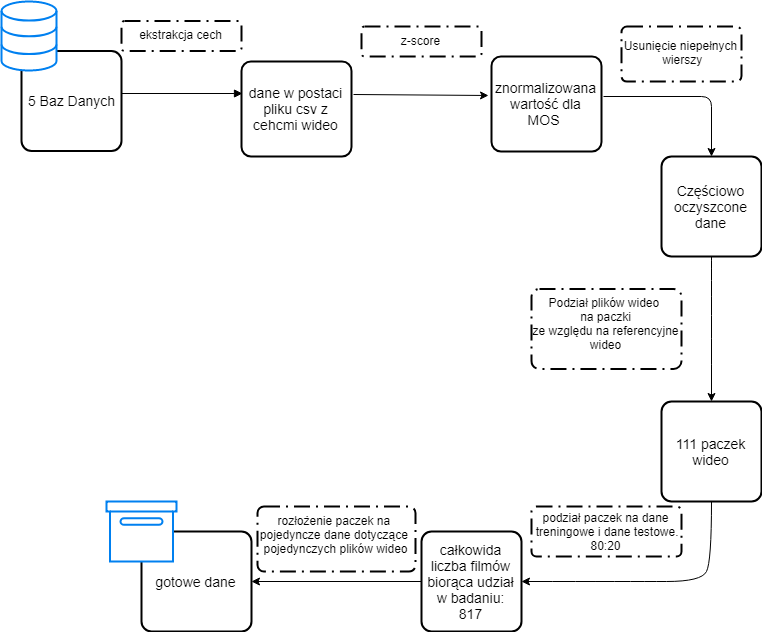
\includegraphics[ height=11cm, width=15cm]{data_preparation_work_flow}
\captionof{figure}{Schemat kroków wykonanych podczas przygotowywania danych.}
\label{fig:data_preparation_work_flow}
\label{fig:xccs}
\end{center}

\subsection{Zbieranie danych}
Rozpoczęcie przetwarzania danych wymaga w pierwszej kolejności ich zebrania. Dla stworzenia algorytmu oceny jakości, podczas wyszukiwania danych, głównym kryterium było odnalezienie takich baz, gdzie oprócz plików wideo (SRC + PVS) istniała również jego subiektywna ocena. Ocena ludzka była konieczna, ponieważ to ona stanowiła dane nadzorcze podczas trenowania modeli. W pracy tej użyto następujące źródła danych:
\begin{itemize}
\item Subjective quality of H.264/SVC videos using ACR-HR method in VGA -- baza danych udostępniona dzięki The Institut de Recherche en Communications et Cybernétique de Nantes. W jej skład wchodzi około 300 plików wideo, ich czas trwania to: 10-12s, a rozdzielczość wszystkich wynosi: 640x480 \cite{pitrey:hal-00608310}.
\item Lab for Video and Image Analysis – LFOVIA -- jest grupą badaczy z Indian Institute of Technology Hyderabad zajmujących się tematyką jakości wideo. Dzięki udostępnionym przez nich plikom,  baza danych wejściowych w niniejszej pracy powiększyła się o 40 nowych obrazów w wysokich rozdzielczościach: FHD (1920x1080), UHD (3840x2160) i czasie trwania po 120 sekund każdy \cite{india}.
\item LIVE Netflix Video Quality of Experience Database -- baza danych stworzona przez naukowców z The University of Texas at Austin. W jej skład wchodzi 26 wideo o rozdzielczości 1920x1080, o długości 120 sekund każdy \cite{netflix_1}\cite{netflix_11}.
\item LIVE-NFLX-II Subjective Video QoE Database -- również stworzona przez The University of Texas at Austin w celu badań nad optymalnym przesyłem wideo w sieci. W bazie danych znajduje się 420 plików wideo o rozdzielczości FHD i czasie trwania około 40 sekund.
\item EPFL-PoliMI video quality assessment database -- Baza plików wideo utworzona przez dwie współpracujące uczelnie: Politecnico di Milano - Włochy i Ecole Polytechnique Fédérale de Lausanne - Szwajcaria. Dane składają się z 12 obrazów referencyjnych (SRC) oraz z aplikacji pozwalającej wygenerować dla nich PVSs. W ten sposób zostały uzyskane około 150 nowych filmów do badań w dwóch rozdzielczościach: 704x576, 352x288 i o czasie trwania około 10s \cite{italy}\cite{italy_2}\cite{italy_3}.
\end{itemize}
Początkowo w badaniach brała udział jeszcze jedna baza wideo z 220-oma plikami. Niestety, jak się okazało plik referencyjny oraz jego zniekształcone wersje posiadały różne wartości fps, przez co metryki typu VMAF nie były w stanie podać miarodajnych wyników. Cała więc baza musiała zostać pominięta.\par

\subsection{Ekstrakcja cech}
Kolejnym krokiem po zebraniu danych była ekstrakcja cech wideo, które później miały być użyte podczas przygotowywania modeli. W celu otrzymania cech należało każde wideo przekształcić do serii pojedynczych ramek w formacie YUV. 

Dalszy proces ekstrakcji był o tyle problematyczny, że różne, do tego wykorzystywane narzędzia, wymagały w różny sposób dostosowanych danych. Co więcej, nieskompresowane wideo zajmuje bardzo dużo przestrzeni dyskowej, a sam proces przetwarzania wideo wymaga również znacznego nakładu pracy dla procesora. Cechy biorące udział w badaniach to: blokowość, aktywność przestrzenna, aktywność czasowa, letterbox, pillarbox, straty bloków, rozmycie, wyciemnienie, zamrożenie, ekspozycja, kontrast, jasność, szum, PSNR, SSIM, MS-SSIM, VMAF, czas trwania, próbkowanie chrominancji, liczba klatek na sekundę.\par

Dane dotyczące metryk $full$-$renerence$ oraz $no$-$reference$ zostały uzyskane na każdą z ramek. W następnym kroku wartości te zostały uśrednione na całe wideo. Wyjątkiem były SSIM i MS\--SSIM tu informacje zostały uzyskane na całe wideo. Cechy pochodzące z obu źródeł: VDK i AGH Video Quality Indicators zostały ujednolicone i zapisane wspólnie w postaci pliku CSV.\par

Dodatkowo w badaniu postanowiono dodać jeszcze jedną cechę, która mogła by mieć wpływ na wynik subiektywny, to znaczy ilość różnych rozdzielczości w bazie. Przykładowo w zestawieniu, w którym pliki posiadają różne rozdzielczości, te z ich wyższą wartością (np. FHD) mogą mocniej kontrastować z tymi o niższej, przez to ocena subiektywna może okazać wyższa. W pracy tej rozpoznano dwa przypadki, kiedy baza danych zawiera pliki o jednej rozdzielczości i baza danych zawiera pliki o dwóch rozdzielczościach. Cecha ta została wprowadzona jako binarna cecha nominalna dla każdego z wideo i odpowiada na pytanie czy plik pochodzi z bazy o jednej rozdzielczości. Jeżeli tak to wartość jej przyjmuje 1, w innym wypadku 0.  \par

Powyższy czynnik jest sztucznie stworzoną cechą, w komercyjnym wykorzystaniu trudną do otrzymania, ponieważ wymagało by to dostępu do obrazów obejrzanych przez widza bezpośrednio wcześniej. Cechę tę można również rozwinąć o inne atrybuty wideo, tak aby móc w lepszy sposób przedstawić różnice pomiędzy ocenianym plikiem, a pozostałą resztą, co leży poza zakresem tego opracowania.\par

Jako dane nadzorujące użyto subiektywną ocenę ludzką.\par

\subsection{Normalizacja i czyszczenie danych}
W zbiorze plików pochodzących od badaczy z Uniwersytetu w Texasie ocena subiektywna została przekazana po znormalizowaniu $z$-$score$, gdzie zakres wartości zawiera się pomiędzy -3 a 3. W celu otrzymania miarodajnych wyników dane z pozostałych baz również zostały w ten sam sposób znormalizowane.\par
Podczas procesu przygotowywania danych jak i późniejszej ekstrakcji cech mogły nastąpić pewne wyjątki, które uniemożliwiły otrzymanie poprawnego wyniku. W takim przypadku cały wiersz dotyczący danego wideo był pomijany podczas tworzenia modeli.

\subsection{Podział danych}

Przy tworzeniu modeli została wykorzystana implementacja algorytmów zawarta w module języka Python -- sklearn. Instancje klas, przedstawiające modele, przyjmują jako dane wejściowe dane w formacie macierzy. Dlatego pliki CSV zostały, podczas działania skryptu, przekształcone do typu DataFarme. Wspierany jest on przez moduł, ułatwiający prace z dużymi danymi -- pandas.\par

Przy eksploatowaniu danych często stosowaną techniką jest $cross$ $validation$. Polega ona na podziale dostępnych danych na dane treningowe i testowe. Można tu wykorzystać zasadę podziału 80:20, co oznacza ze 80 części danych jest przeznaczonych na dane treningowe, a 20 na dane testujące. Dobrą praktyką jest, aby w obu z tych grup znalazły się dane z całego przekroju bazy danych. Zabieg ten ma na celu pozwolenie na identyfikacje  problemu generalizacji czy nad dopasowania. 

W przedstawionej pracy proces podziału danych należało przeprowadzić, tak aby uwzględnić  całe grupy --  SRC i jego PSV. Dane z jednej takiej grupy powinny w całości znaleźć się w podzbiorze danych testowych bądź treningowych. Nie zastosowanie tego zabiegu mogło by poskutkować niemiarodajnym wysokim wynikiem R-kwadrat. Wysoki R-kwadrat powinien wskazywać na dużą trafność modelu. Jednak w tym przypadku oznaczało by to, że odnajduje on zależności związane z grupami wideo, które wzięły udział w tym badaniu. Zaproponowany tu podział pozwala na uniknięcie tego niepożądanego efektu. Schemat podziału jest przedstawiony na rysunku \ref{fig:podzial_danych}.

\begin{center}
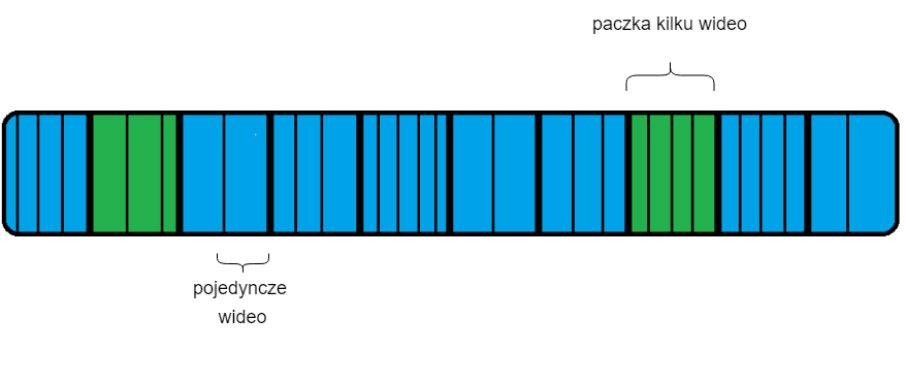
\includegraphics[ height=5cm, width=10cm]{podzial_danych}
\captionof{figure}{Przykładowy podział danych na dane testowe i treningowe (80:20). Niebieskie prostokąty odnoszą się do danych treningowych, a zielone do danych testowych.}
\label{fig:podzial_danych}
\label{fig:xccs}
\end{center}
Ostatnim etapem podczas przygotowywania danych było połączanie elementów z każdej z grup. Od tego momentu wektor danych wejściowych podczas przygotowywania modelu odnosi się do pojedynczego pliku wideo.


\clearpage

\subsection{Podsumowanie danych}
Poniższa tabela \ref{tab:tabela} przedstawia uzyskane dane 


\begin{table}[!hbp]
\centering
\begin{tabular}{|c|l|l|l|l|}
\hline
\multicolumn{5}{|c|}{5 baz danych, ponad 800 wektorów danych, ponad 100 paczek plików wideo} \\ \hline
\multicolumn{5}{|c|}{21 cech statystycznych} \\ \hline
\multicolumn{2}{|c|}{ilościowe} & \multicolumn{3}{c|}{jakościowe} \\ \hline
\multicolumn{2}{|l|}{\begin{tabular}[c]{@{}l@{}}blokowość, aktywność przestrzenna, aktywność czasowa,\\ letterbox, pillarbox, straty bloków, rozmycie, wyciemnienie, \\ zamrożenie, ekspozycja, kontrast, jasność, szum, \\ PSNR, SSIM, MS-SSIM, VMAF, czas trwania,\end{tabular}} & \multicolumn{3}{l|}{\begin{tabular}[c]{@{}l@{}}próbkowanie chrominancji,\\ rozdzielczość, \\ liczba dostępnych rozdzielczości\end{tabular}} \\ \hline
\end{tabular}
\caption{Podsumowanie przygotowania danych}
\label{tab:tabela}
\end{table}





\section{Proces budowania i testowania modeli}
\label{cha:drugiDokument}


Z uwagi na specyfikę przygotowania danych treningowych i testowych każdy z modeli został zbudowany i przetestowany wiele razy. Każdorazowe wykonanie tej operacji generuje zbiór modeli dla każdego sprawdzanego algorytmu na każdy testowany zestaw danych. Poniższy akapit tłumaczy potrzebę tego zabiegu.

Podział danych 80:20 dotyczy paczek SRC + PSV, natomiast budowa modeli odbywa się już na podstawie danych z pojedynczych plików wideo. Dlatego może zaistnieć sytuacja kiedy większość małych paczek (na przykład po tylko 3 pliki wideo) znajdą się w danych treningowych, a większość dużych (na przykład po 15 wideo) w danych testujących. Tym samym faktyczny podział może wynosić w skrajnym przypadku 50:50, zamiast 80:20 (taki sam odstęp może wystąpić w drugą stronę). Dlatego  przy  każdym uruchomieniu aplikacji, podział zgromadzonych danych dobywał się na zasadzie losowo wybranych paczek do każdej grup -- danych trenujących i testujących, przy zachowaniu podziału 80:20.\par

Wykres \ref{fig:execution} odnosi się do przeprowadzonego eksperymentu, który pomógł wybrać optymalną liczbę iteracji dla wyżej omówionej techniki. Linie przedstawia uśrednione R-kwadrat na liczbę modeli(w tym przypadku powstałych na bazie zestawu danych wejściowych numer 18 -- tabela 3.2) biorących udział podczas jej obliczania. Czytając ten wykres można stwierdzić, że dla każdego z algorytmów wyniki  stabilizują się przy około 80 modelach. W celu uniknięcia niemiarodajnych wyników w dalszych badaniach  wybrano liczbę (z pewnym zapasem) stu modeli na podstawie których  obliczany był uśredniony R-kwadrat.

\begin{center}
	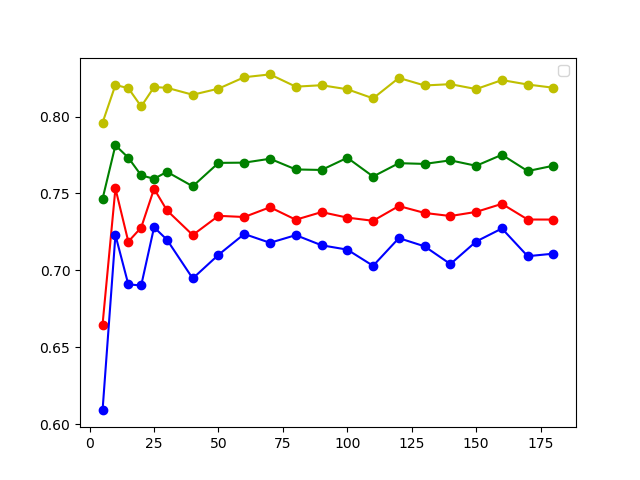
\includegraphics[ height=7cm, width=11cm]{execution}
	\captionof{figure}{Uśredniony R-kwadrat na liczbę modeli biorących udział w jego liczeniu. Badanie dla zestawu 18 z tabeli 3.2.}
	\label{fig:execution}
	\label{fig:xccs}
\end{center}

W badaniach postanowiono sprawdzić  modele trenowane w oparciu o: każdą z osobna metrykę FR, wybrane metryki NR i ich niektóre kombinacje. Uruchomienia sekwencji budowania i testowania odbywały się na zestawach cech prezentowanych w tabeli 3.2.  Dalsze rozdziały będą odnosić się do poniższej numeracji w kontekście zestawów cech.

\begin{table}[]
	\raggedright
	\begin{tabular}{|l|l|}
		\hline
		\textbf{\begin{tabular}[c]{@{}l@{}}Numer \\ zestawu\end{tabular}} & \textbf{Cechy}                                                                                                                                                                                                                                                                 \\ \hline
		1                                                                 & VMAF                                                                                                                                                                                                                                                                           \\ \hline
		2                                                                 & VMAF, SSIM                                                                                                                                                                                                                                                                     \\ \hline
		3                                                                 & MS-SSIM                                                                                                                                                                                                                                                                        \\ \hline
		4                                                                 & PSNR                                                                                                                                                                                                                                                                           \\ \hline
		5                                                                 & PSNR, VMAF                                                                                                                                                                                                                                                                     \\ \hline
		6                                                                 & PSNR, VMAF, SSIM, MS-SSIM                                                                                                                                                                                                                                                      \\ \hline
		7                                                                 & \begin{tabular}[c]{@{}l@{}}PSNR, VMAF, SSIM, MS-SSIM, blokowość, aktywność przestrzenna, pillarbox, \\ straty bloków, rozmycie, aktywność czasowa, wyciemnienie, ekspozycja, kontrast, \\ jasność, czas trwania, rozdzielczości\end{tabular}                                   \\ \hline
		8                                                                 & \begin{tabular}[c]{@{}l@{}}PSNR, VMAF, SSIM, MS-SSIM, blokowość, aktywność przestrzenna, pillarbox, straty bloków, \\ rozmycie, aktywność czasowa, wyciemnienie, ekspozycja, kontrast, jasność, czas trwania, rozdzielczości, \\ liczba dostępnych rozdzielczości\end{tabular} \\ \hline
		9                                                                 & PSNR, VMAF, SSIM, MS-SSIM, rozmycie, straty bloków                                                                                                                                                                                                                             \\ \hline
		10                                                                & PSNR, VMAF, SSIM, MS-SSIM, rozmycie, straty bloków, liczba dostępnych rozdzielczości                                                                                                                                                                                           \\ \hline
		11                                                                & PSNR, VMAF, SSIM, MS-SSIM, jasność                                                                                                                                                                                                                                             \\ \hline
		12                                                                & PSNR, VMAF, SSIM, MS-SSIM, jasność, blokowość, straty bloków, rozmycie                                                                                                                                                                                                         \\ \hline
		13                                                                & \begin{tabular}[c]{@{}l@{}}PSNR, VMAF, SSIM, MS-SSIM, jasność, blokowość, straty bloków, rozmycie, \\ liczba dostępnych rozdzielczości\end{tabular}                                                                                                                            \\ \hline
		14                                                                & PSNR, VMAF, SSIM, MS-SSIM, jasność, ekspozycja                                                                                                                                                                                                                                 \\ \hline
		15                                                                & PSNR, VMAF, SSIM, MS-SSIM, jasność, ekspozycja, liczba dostępnych rozdzielczości                                                                                                                                                                                               \\ \hline
		16                                                                & PSNR, VMAF, SSIM, MS-SSIM, jasność, liczba dostępnych rozdzielczości                                                                                                                                                                                                           \\ \hline
		17                                                                & PSNR, VMAF, SSIM, MS-SSIM, czas trwania                                                                                                                                                                                                                                        \\ \hline
		18                                                                & PSNR, VMAF, SSIM, MS-SSIM, czas trwania, liczba dostępnych rozdzielczości                                                                                                                                                                                                      \\ \hline
		19                                                                & \begin{tabular}[c]{@{}l@{}}PSNR, VMAF, SSIM, MS-SSIM, czas trwania, liczba dostępnych rozdzielczości,\\  rozdzielczości\end{tabular}                                                                                                                                           \\ \hline
		20                                                                & PSNR, SSIM                                                                                                                                                                                                                                                                     \\ \hline
		21                                                                & SSIM                                                                                                                                                                                                                                                                           \\ \hline
		22                                                                & blokowość                                                                                                                                                                                                                                                                      \\ \hline
		23                                                                & \begin{tabular}[c]{@{}l@{}}blokowość, aktywność przestrzenna, pillarbox, straty bloków, rozmycie, aktywność czasowa,\\  wyciemnienie, ekspozycja, kontrast, jasność, rozdzielczości, liczba dostępnych rozdzielczości\end{tabular}                                             \\ \hline
		24                                                                & \begin{tabular}[c]{@{}l@{}}blokowość, aktywność przestrzenna, pillarbox, straty bloków, rozmycie, aktywność czasowa, \\ wyciemnienie, ekspozycja, kontrast, jasność, czas trwania, rozdzielczości\end{tabular}                                                                 \\ \hline
		25                                                                & \begin{tabular}[c]{@{}l@{}}blokowość, aktywność przestrzenna, pillarbox, straty bloków, rozmycie, aktywność czasowa,\\ wyciemnienie, ekspozycja,  kontrast, jasność, czas trwania, rozdzielczości, liczba dostępnych rozdzielczości\end{tabular}                               \\ \hline
		26                                                                & straty bloków                                                                                                                                                                                                                                                                  \\ \hline
		27                                                                & rozmycie                                                                                                                                                                                                                                                                       \\ \hline
		28                                                                & jasność                                                                                                                                                                                                                                                                        \\ \hline
		29                                                                & kontrast                                                                                                                                                                                                                                                                       \\ \hline
		30                                                                & ekspozycja                                                                                                                                                                                                                                                                     \\ \hline
	\end{tabular}
	\caption{Numeracja zestawów danych biorących udział w badaniu.}
	\label{tab:tabela2}
\end{table}
\AddThispageHook{\thispagestyle{empty}}%

\clearpage
\section{Modele }
\label{cha:drugiDokument}


W niniejszej pracy zostały przetestowane cztery algorytmy uczenia maszynowego przedstawione w części teoretycznej. Parametry definiujące ich działanie zostały dobrane na zasadzie obserwacji kolejnych prób i wiedzy na temat ich działania. W ten sposób zostały wyselekcjonowane poniższe parametry, które pozwoliły na osiągnięcie najwyższego wskaźnika R-kwadrat dla jednego z zestawów cech.  \par

Regresja liniowa została sprawdzona w pierwszej kolejności. Jako referencyjny i jeden prostszych z algorytmów, nie wymaga ona podania dodatkowych parametrów, aby zadziałał w prawidłowy sposób. W tym przypadku wektor danych wejściowych podczas trenowania przedstawia się  następująco \ref{eqn:regresja}, gdzie $y_i$ jest subiektywną oceną dla filmu $i$, a $x_{1i}, x_{2i}...$ są jego cechami. \par

Kolejnym testowanym algorytmem był SVR. Użyta funkcja kernela do wyznaczenia hiperpłaszczyzny to $Radial$ $Basis$ $Function$ (RBF). Współczynnikowi $\epsilon$ została przypisana wartość $0,1$. Przy współczynniku $\gamma$, który mówi jak odległe punkty będą miały wpływ na budowaną hiperpłaszczyznę, skorzystano z metody już zaimplementowanej w pakiecie sklearn, pozwalającej na wyznaczenie bardziej dopasowanej wartości, bazując na dostępnym zbiorze danych. Parametr $C$, który odpowiada za wygładzenie funkcji SVR wynosi 0.7.\par
%https://www.ncbi.nlm.nih.gov/pmc/articles/PMC2839056/

Las losowy działa w oparciu o parametry podane przez badacza, takie jakie jak ilość drzew i ich głębokość. W tym przypadku użyto 100 drzew o głębokości 8. Jako metodę podejmowania decyzji o podziale danych (tworzenia węzłów decyzyjnych), został wybrany \emph{Gini Index}. \par

Ostatnim sprawdzonym algorytmem uczenia maszynowego była sieć neuronowa z następującymi parametrami -- 3 warstw ukrytych po 13 neuronów w każdej. Maksymalna ilość iteracji algorytmu $Backward$ $Propagation$ po której model będzie gotowy to 1000. Parametr $learning$ $rate$, określający szybkość uczenia, został ustawiony na wartość 0,001. Natomiast funkcję aktywacji stanowiła funkcja ReLU.\par





\chapter{Wyniki i ich analiza }
Poniższy rozdział prezentuje wyniki testów z poszczególnych modeli. Zostały one zebrane na wykresie słupkowym \ref{fig:podsumowanie}, gdzie oś x odnosi się do numerów zestawów, a oś y do średnich wartości R-kwadrat. Wyniki tu przedstawione dotyczą algorytmów z ostatecznie wybranymi parametrami. 

Selekcja tych parametrów dla  każdego z algorytmów została dokonana na podstawie najlepszego osiągniętego dopasowania. Przykładowo dla  sieci neuronowych testowane były konfiguracje: 2 warstwy ukryte i 8 neuronów, 4 warstwy ukryte i 13 neuronów, 3 warstwy i ukryte 13 neuronów (z różnymi współczynnikami uczenia i funkcjami aktywacji)\todo{było jeszcze kilka innych, ale nie chce zbytnio o tym pisać, bo niektóre testy to na zasadzie kolejnego uruchamiania i obserwacji } W oparciu o każdą z nich budowano modele, na zasadzie opisanej w poprzednim rozdziale,  dla każdego z wcześniej zdefiniowanych zestawów.  Najwyższy średni R-kwadrat został osiągnięty dla ostatniej z wymienionych konfiguracji i dla zestawu 19. Tak więc prezentowane wyniki na wykresie  \ref{fig:podsumowanie} będą odnosić się do tych właśnie parametrów. Taki wykres pozwala czytelnikowi odczytać najistotniejszą dla tej pracy informację o najtrafniejszym z modeli, oraz dodatkowo prezentuje inne zjawiska związane z eksploracją danych. Co więcej wyniki z innych testowanych konfiguracji algorytmów uczenia maszynowego nie odbiegały znacząco od tych zaprezentowanych na obecnym wykresie. W dalszej części rozdziału  odbędzie się jego analiza.
 
    



\begin{sidewaysfigure}[ht]
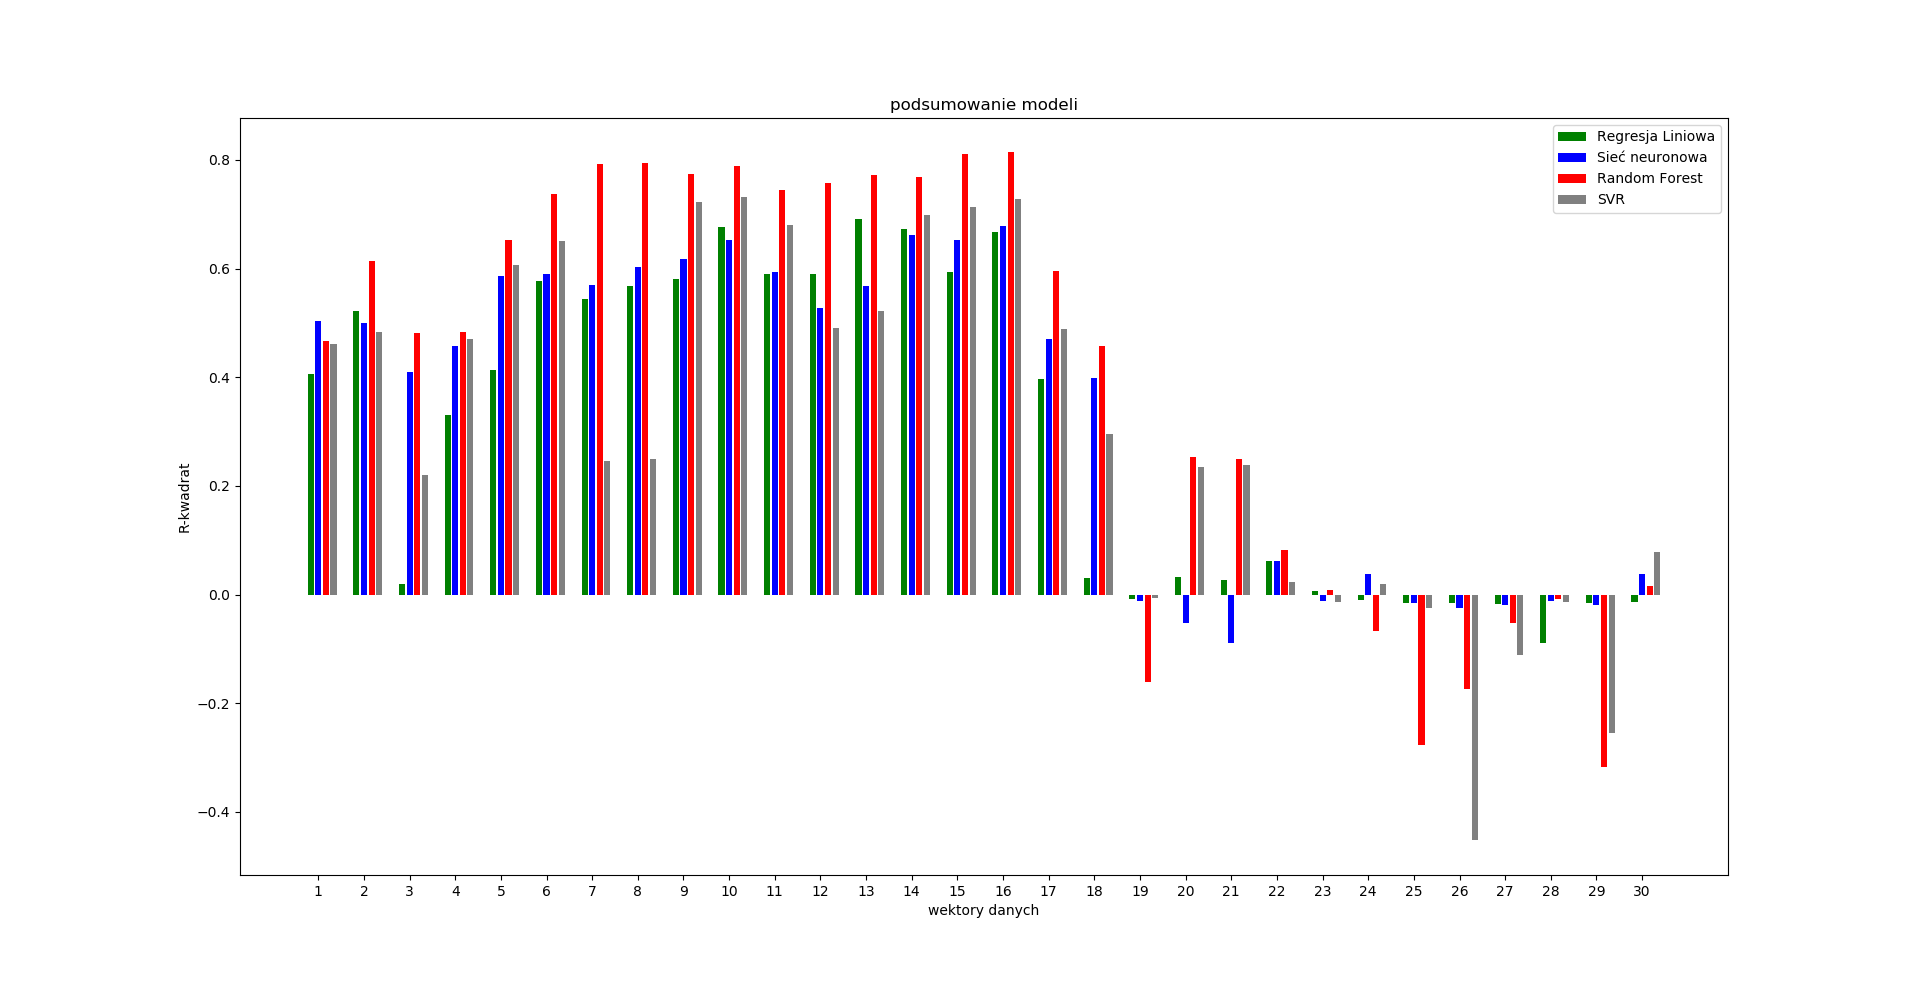
\includegraphics[ height=15cm, width=26cm]{podsumowanie}
\captionof{figure}{Wyniki z poszczególnych modeli}
\label{fig:podsumowanie}
\label{fig:xccs}
\end{sidewaysfigure}

W pierwszej kolejności wyjaśniane zostaną różnice w obrębie zestawów danych, a pomiędzy poszczególnymi modelami. Czyli przykładowo: "Dlaczego dla zestawu 17 różne algorytmy dają róże wyniki?".  Różnice te wynikać mogą z charakterystyki testowanych algorytmów uczenia maszynowego. Niektóre z nich potrafią odnaleźć fałszywe zależności w danych treningowych, które nie wystąpiły w czasie testów, czyli występuje  nad-dopasowanie dla pewnych cech. Inną przyczyną może być generalizacja, przez którą może nastąpić pominięcie pewnych informacji ukrytych w danych. Każdy z algorytmów przejawia różne właściwości dopasowania do dostępnych danych, Co przekłada się na różne poziomy trafności modelów.    \par

Obserwując  poszczególne wyniki dla zestawów $no$-$reference$ (22 -- 30)  oraz $full$-$reference$ (1 -- 6, 20, 21) można zaobserwować, że te drugie znacznie trafniej dokonują predykcji. Prawdopodobną przyczyną występowania tej sytuacji jest nierównomierność w występowaniu cechy typu NR w dostępnych danych, co może dalej skutkować niewłaściwym dopasowaniem  modelu. Wysoki wyniki metryk FR dodatkowo potwierdzał by powszechną opinię o lepszej skuteczności tych wskaźników jakości.

Obserwacja wyników wykazała również, że wprowadzona dodatkowa cecha (liczba dostępnych rozdzielczości)  ma  wpływ na ocenę jakość, choć w niewielkim stopniu.  W większości przypadków zestaw z tą cecha otrzymywał wyższe R-kwadrat, niż ten sam zestaw ale bez liczby dostępnych zależności. Wykres kołowy \ref{tab:tabela rozdzielczosc} przedstawia w jakiej części przypadków dana obserwacja się powtarza.\todo{ Podobne sprawdzone tu oddziaływanie to czas trwania. Dla dłuższych wideo  modele daje lepsze wyniki, różnice również są nieznaczne.} \par

\begin{center}
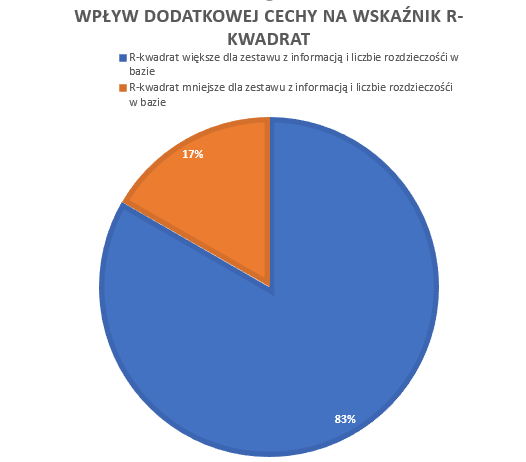
\includegraphics[ height=8cm, width=10cm]{w_kolowy}
\captionof{figure}{Wykres przedstawia stosunek liczby modeli zbudowanych z zestawów z dodatkową cechą, ocenionych jako bardziej trafnych, do liczby przypadków kiedy taki model został oceniony jako gorszy. W 40 przypadkach oceniony, jako lepszy 8 jako gorszy. Rozwarzane zestawy to pary: 14 i 15, 17 i 18, 7 i 8, 11 i 16, 9 i 10, 24 i 25.}
\label{tab:tabela rozdzielczosc}
\label{fig:xccs}
\end{center}
 
%zestawy: 14 i 15, 17 i 18, 7 i 8, 11 i 16, 9 i 10, 24 i 25 są dla siebie bliźniacze z różnicą dodatkowej cechy. Zestawy oznaczone * zawierają dodatkową ceche. Zielony kolor wskazuję na pole z większym R-kwadrat na pare, czerwony na mniejszy(test powtórzony dwa razy). 
\topskip0pt
\vspace*{\fill}  
Na wykresie \ref{fig:podsumowanie} można dostrzec, że różnice pomiędzy modelami zbudowanymi na podstawie zestawów: 18, 19, 17, 8, 7, 10, 13, 15, 9, 16, 12, 14, 11, 6  wyróżniają się pod kątem wysokich wartości R-kwadrat. Dla tych zestawów wspólnym mianownikiem są cechy: PSNR, VMAF, SSIM, MS-SSIM. Każda cecha z osobna również osiąga wysokie wyniki (Przykładowo, R-kwadrat kolejno dla modelu Lasu Losowego: 0.490, 0.502,  0.475,  0.507). Niższe jednak niż te osiągnięte w zestawie. 
Wymienione wyżej cechy posiadają wysoki współczynnik korelacji \ref{fig:korelacja}, przez co łączenie ich tylko w pewnym stopniu poprawia trafność modelu. Końcowa wartość nie jest ich sumą. Przykładowo dla zestawu 2 (VMAF + SSIM) R-kwadrat wynosi 0.636 \par
\vspace*{\fill}


\begin{center}
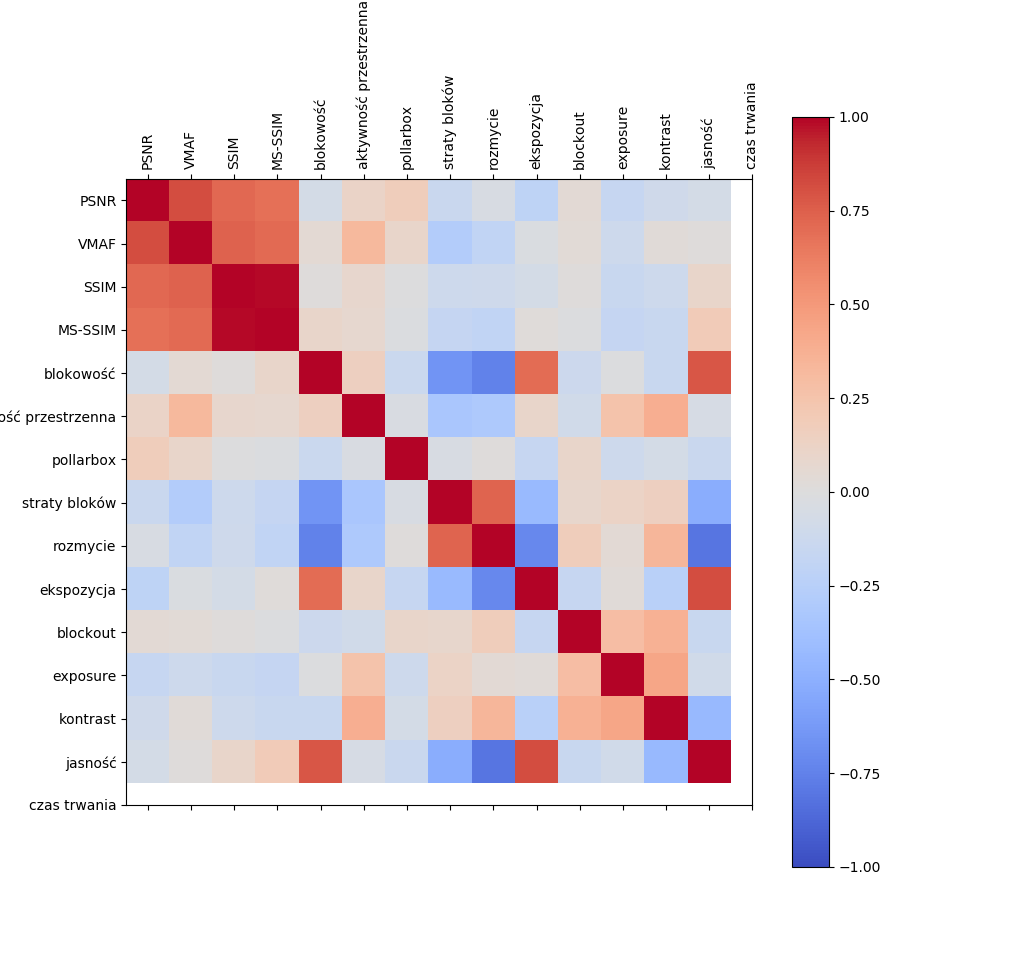
\includegraphics[ height=14cm, width=14cm]{korelacja}
\captionof{figure}{Korelacja pomiędzy poszczególnymi cechami.}
\label{fig:korelacja}
\label{fig:xccs}
\end{center}



\topskip0pt
\vspace*{\fill} 
Kolejny aspekt, który można odnotować czytając wykres \ref{fig:podsumowanie}, to ujemna wartość R-kwadrat dla niektórych zestawów. Biorąc pod uwagę wzór \ref{eqn:r2}, zauważyć należy to, że model podczas testów dokonywał gorszej predykcji, niż średnia dla zbioru danych testowych. Tą sytuację przedstawia wykres \ref{fig:kontrast_ujemne_rk}. Zaprezentowane są tu próbki danych dla cechy kontrast. Funkcja regresji liniowej (linia niebieska)  pokrywa się ze średnią dla danych testowych (linia pomarańczowa), ale podczas liczenia R-kwadrat brana pod uwagę jest średnia ze zbioru danych testowych (linia czerwona). Gdyby ta ostania pokrywała się z linią regresji R-kwadrat wynosił by 0. Ujemny, R-kwadrat oznacza również, że dla danej cechy lub ich zestawu, algorytm nie odnalazł zależności między zmiennymi opisującymi, a zmienną opisywaną.\par
\vspace*{\fill}

\begin{center}
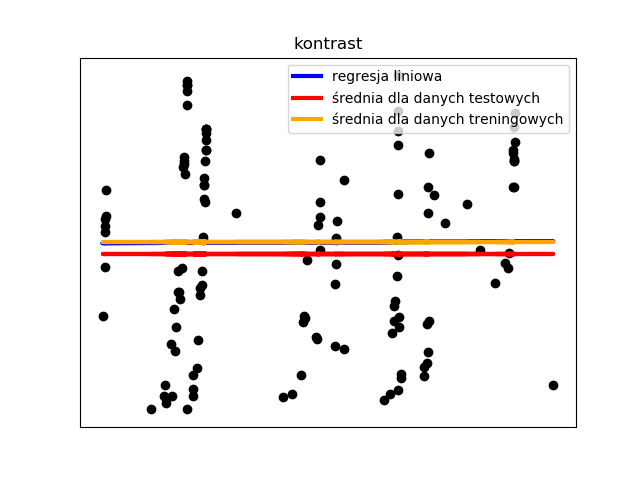
\includegraphics[ height=10cm, width=13cm]{kontrast_ujemne_rk}
\captionof{figure}{Przypadek kiedy wskaźnik r-kwadrat jest ujemny.}
\label{fig:kontrast_ujemne_rk}
\label{fig:xccs}
\end{center}

Najwyższy uśredniony wynik R-kwadrat został osiągnięty przez modele zbudowane na podstawie algorytmu \textbf{lasu losowego} (z zadanymi wcześniej parametrami) z użyciem \textbf{zestawu 18}, czyli \textbf{0.824}. Zestaw ten składa się z  zebranych metryk full-reference z uwzględnieniem czasu trwania wideo i dodatkowej cechy dotyczącej ilości dostępnych rozdzielczości. Każdy z modeli z tej grupy daje nieco inne  wyniki (odchylenie standardowe wynosi 0.053, jest stosunkowo nieduże w porównaniu z innymi modelami i zestawami) ponieważ budowany jest na różnych próbkach danych.  Odnosząc się do tematu pracy, ma on największe szanse na trafne wyznaczenie jakość wideo. Podobnie jak [link do badan robionych w podobny sposób]\todo{text}i w tym przypadku jako szukany model należy uznać jeden ze stu modeli dla tych/tu wyróżnionych parametrów. 




\chapter{Podsumowanie}

\todo{ewentualnie -  dodac sprawdzenei mojej metryki z wskaznikiem koralacji Pearson'a, jezeli > 0.9 to dobra metryka }


Prezentowana praca stawiała sobie za cel stworzenie algorytmu oceniającego jakość wideo.

Po uprzednim przygotowaniu danych, do dyspozycji badającego były informacje opisujące wideo –- zarówno metryki FR jak i NR. Metryki zostały wykorzystane do zbudowania i przystosowania czterech pul modeli w oparciu o  cztery algorytmy uczenia maszynowego. Wykreowane modele mogą posłużyć jako algorytmy oceniające jakość wideo.

Zmierzając do zniwelowania różnic wynikających ze specyficznego podziału danych stworzono ponad 100 modeli dla każdego z algorytmów, gdzie, na podstawie uśrednionego wyniku R-kwadrat, został wybrany optymalny algorytm (wraz z parametrami) i zestaw cech - jako dane wejściowe. Odnosząc się do tematu pracy, algorytmem oceniającym jakość jest jeden z modeli przygotowany w oparciu o wyżej wymienione czynniki -- Las Losowy składający się z 100 drzew o głębokości 8 wraz cechami z zestawu 18 [link do zserializowanego modelu].\todo{text}

Co więcej, można postawić tezę, że chociaż wszystkie metryki FR, w tym badaniu, mają wysokie wartości R-kwadrat, to jednak możliwa jest sytuacja, kiedy ich ocena znacząco będzie odbiegać od SQV. Wideo referencyjne może już na samym początku może być zniekształcone poprzez nieprawidłowe nagranie. Policzony wtedy PSNR dla SRC i PVS wykaże wysoką jakość obrazu ale ocena odbiorcy będzie negatywna.

Przedstawione w obecnym studium rozwiązanie nie jest uniwersalnym wyznacznikiem jakości wideo. Z pewnością mogą istnieć czynniki, które nie zostały w pracy uwzględnione. Z faktu, że badanie korzysta z oceny ludzkiej jako cechy nadzorującej mogą wynikać nie brane pod uwagę efekty zmieniające tę ocenę.

Należy stwierdzić, że z biegiem lat oczekiwania co do jakości wideo znacznie rosną. Chociaż w latach 90 ubiegłego wieku tamtejsze wideo uznawane było jako produkt wysokiej klasy, to współcześni widzowie nie byliby w żaden sposób usatysfakcjonowani odbiorem takiego obrazu. 

Dodatkowo, biorąc dynamicznie rozwijający się rynek multimediów, warto zwrócić uwagę na nowe technologie jeszcze nie tak mocno spopularyzowane. Dla nich może się okazać, że żadna do tej pory dostępnych metryk, również ta  zaproponowana w niniejszej pracy,  nie spełnia oczekiwań. Przykładowo niebrany do tej pory pod uwagę w czasie badań rodzaj wideo wykorzystywana w VR (\textit{ang. Virtual Reality}) -- wideo 360.  

Przeprowadzone badania i zebrane dane mogą posłużyć do dalszych bardziej
zaawansowanych studiów nad jakością wideo. Przykładowo mogły by one uwzględniać aktualny rodzaj zniekształceń i warunków odbioru dla widza i na tej podstawie stworzyć metrykę, która dostosowuje się do tak zadanej sytuacji.


\label{cha:pierwszyDokument}










%\include{tests}



% itd.
% \appendix
% \include{dodatekA}
% \include{dodatekB}
% itd.


\printbibliography
\addcontentsline{toc}{chapter}{Bibliografia}

\end{document}
